\subsection{Betrachtung einzelner Werke}
\hypertarget{RefHeadingToc100333752}{}

\subsubsection{Weihegesang Es-Dur}

\label{bkm:Ref100062450}\hypertarget{RefHeadingToc100333753}{}\label{bkm:Ref100062461}\label{bkm:Ref100062456}Nationalsozialistische
Musik war eine Facette von Högns Schaffens, was der Weihegesang Es-Dur
unweigerlich deutlich (siehe auch \ref{bkm:Ref99597687} „Högn und der
Nationalsozialismus“, Seite \pageref{bkm:Ref99597697}). Nur zu gerne
möchte man angesichts der dunklen Geschichte Deutschlands im 3. Reich
nicht nur die historischen Ereignisse vergessen, sondern auch die von
den Nazis zur Massenmanipulation benutzte Propagandamusik. Im
Vordergrund der Betrachtung soll stehen, inwiefern sich Högn beim
Weihegesang kompositorischer Mittel bedient, die er vor allem in seinen
geistlichen Werken einsetzt. Schon die Tatsache, dass der Weihegesang
bei den weltlichen Trauerfeiern für gefallene Soldaten eine ähnliche
Funktion wie Högns Grablieder bei christlichen Beerdigungen einnahm,
drängt einen Vergleich des Weihegesangs mit seinen Grabliedern auf. Dem
Weihegesang, er wurde wahrscheinlich am Kriegerdenkmal
gesungen, \footnote{Interview Nr. 6, Wilhelm Ederer, 2.1.2003, Absatz
6} fiel gewissermaßen eine Ersatzfunktion für das am Grab bei einer
Beerdigung gesungene Grablied zu. Zum Vergleich wird nicht das Grablied
Nr. 4 von Högn herangezogen. Das Grablied Nr. 4 unterscheidet sich von
den Grabliedern Nr. 1 – 3 sowohl im Aufbau als auch in der Besetzung.
Mit der Besetzung für Sopran-Solo, Chor und Orgel kam das Grablied Nr.
4 nicht im Freien am Grab, sondern in der Kirche beim Requiem zu
Einsatz.

\begin{center}
\begin{minipage}{6.969cm}
\begin{center}
\tablefirsthead{}
\tablehead{}
\tabletail{}
\tablelasttail{}
\begin{supertabular}{m{6.769cm}}

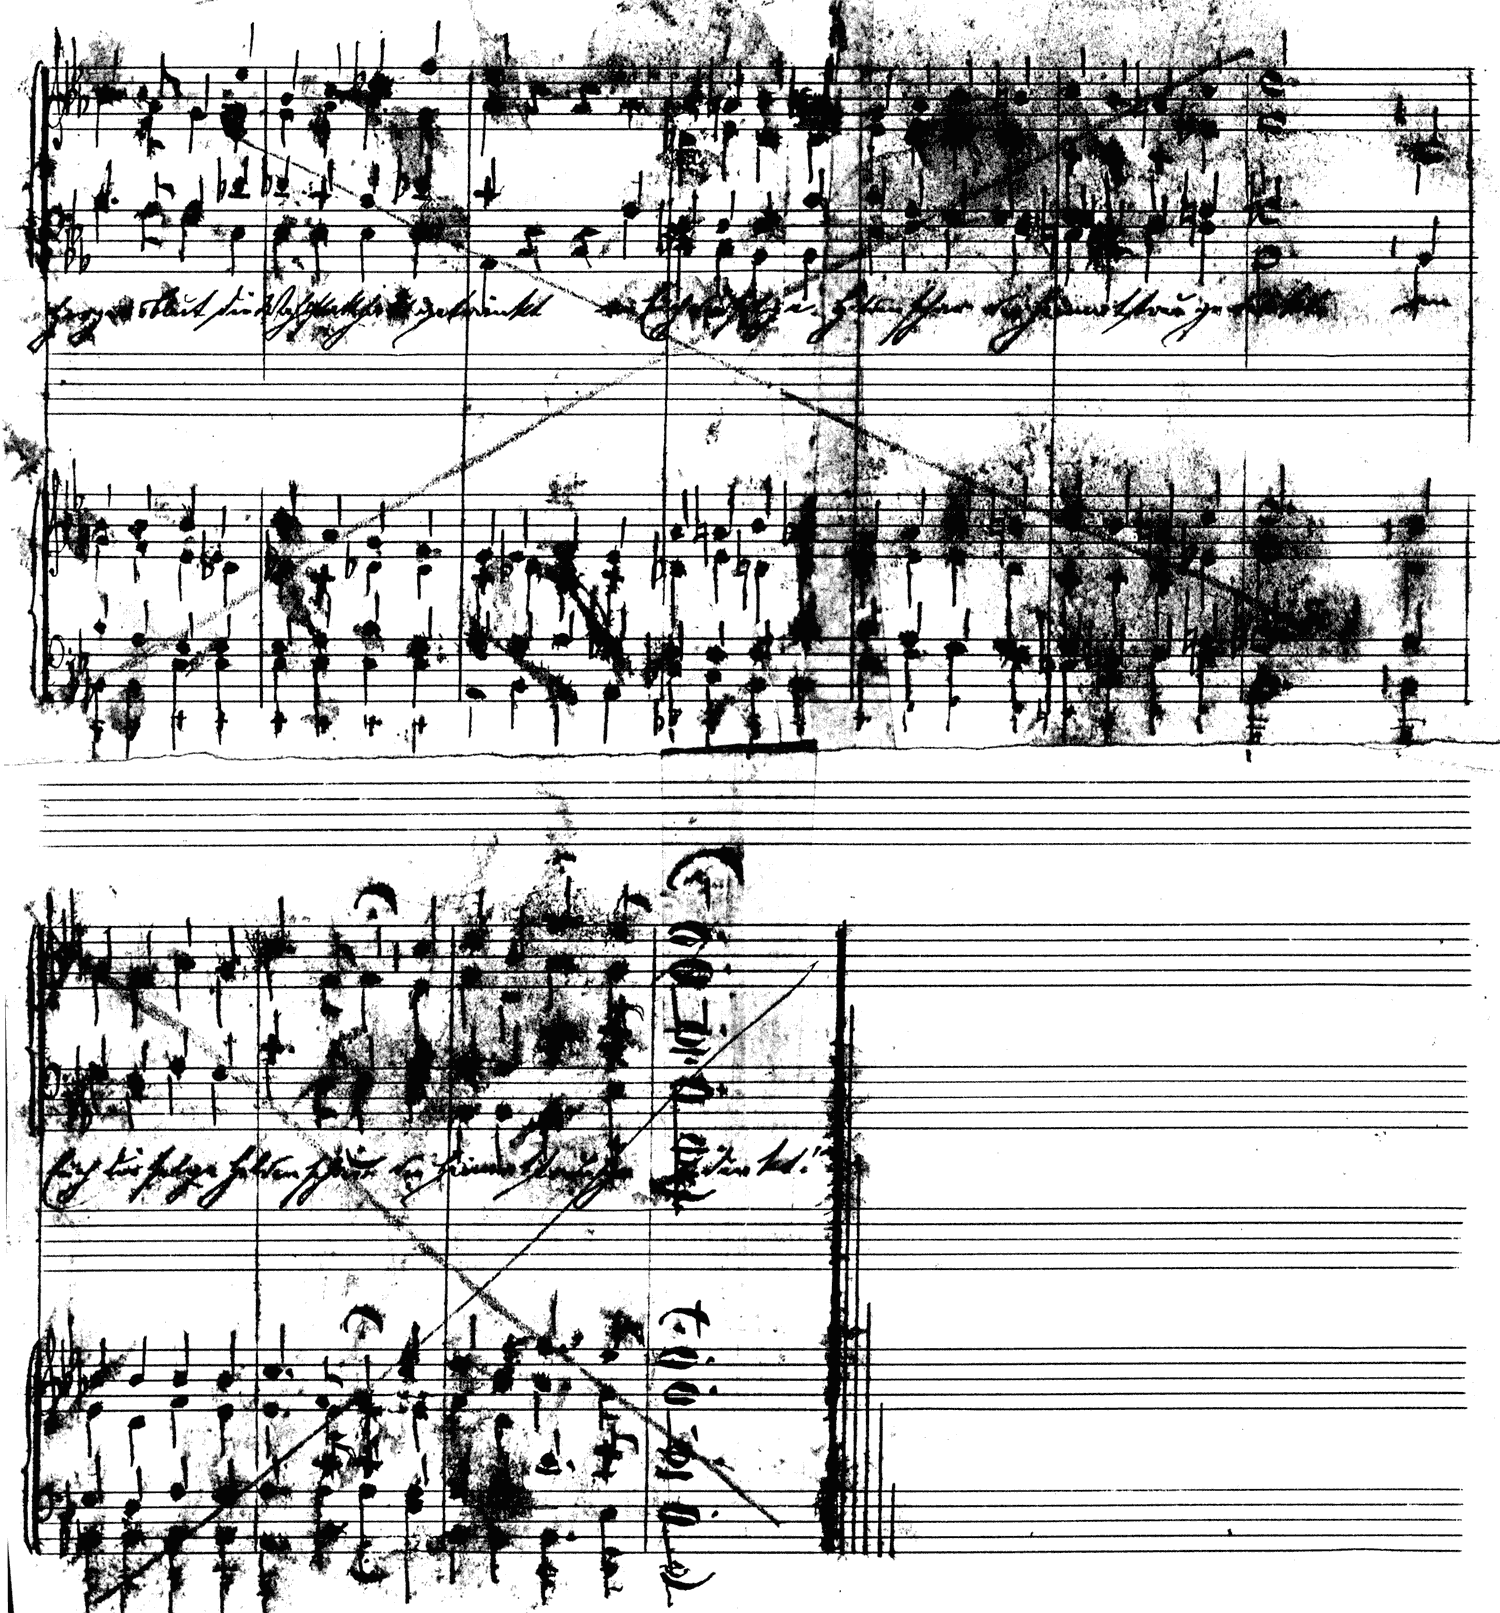
\includegraphics[width=6.588cm,height=7.084cm]{pictures/zulassungsarbeit-img102.png}

Abb. \stepcounter{Abb}{\theAbb}: Weihegesang Es-Dur, Ausschnitt aus der
fragmentarisch erhaltene Partitur\\
\end{supertabular}
\end{center}
\end{minipage}
\end{center}
Kaum Unterschiede im musikalischen Aufbau des Weihegesangs (siehe Band
III, Seite 94 – 95) sind im Vergleich zu den Grabliedern Nr. 1 – 3
(siehe Band III, 80 – 86) zu erkennen. Mit anderen Worten: Hätte die
Musik des Weihegesangs einen geistlichen Text unterlegt, würde sich das
neu entstandene Stück gut in das Bild des Genres passen, das die
Grabliedern Nr. 1 – 3 suggerieren. Alle vier Stücke stehen in Es-Dur,
sind für vierstimmigen Chor mit vierstimmiger Blechbläserbegleitung
geschrieben und haben vier Takte Instrumentalvorspiel. Wie die drei
erwähnten Grablieder ist auch der Chorsatz des Weihegesangs
ausschließlich homophon angelegt und alle vier Gesangstimmen sind
permanent beim Choreinsatz vertreten. Der Blechbläserbegleitung fällt
in den Grabliedern Nr. 1 – 3 und im Weihegesang nicht nur einleitend,
begleitende sondern auch überleitende Funktion zu. Die
Instrumentalbegleitung schließt in allen zuvor genannten Stücken die
klanglichen Lücken, die im Chorsatz beim Phrasenübergang entstehen und
schafft so eine Verbindung von Phrase zu Phrase. Im Gegensatz zu den
Grabliedern spielt das Bläserquartett im Weihegesang immer und pausiert
nicht mehrere Takte wie in den Grabliedern. \newline
Ebenso hat der Weihegesang eine farbige und lieblich wirkende Harmonik
mit den Grabliedern Nr. 1 – 3 gemeinsam. Der in den Grabliedern Nr. 1 –
3 oft verwendete dominantische kleine Septnonakkord (z. B. Grablied Nr.
1 Takt 25, Grablied Nr. 2 Takt 7, Grablied Nr. 3 Takt 17) trägt auch im
Weihegesang in den Takten 6, 12 und 16 maßgeblich zur lieblich, wenn
nicht sogar teilweise kitschig erscheinenden Harmonik bei. Sogar an
einer textlich wie musikalisch exponierten Stelle setzt Högn unter eine
Fermate im Takt 23 einen kleinen Mollseptakkord im Weihegesang, einen
Akkord der wie im Grablied Nr. 1 in Takt 7 den Satz harmonisch
erweitert und ihm einen weichen Charakter verleiht. Auch die zwei
Unisono-Stellen des Chores ändern wenig am lieblichen Gesamtcharakter
des Weihegesangs. Mit dem Grablied Nr. 3 weist der Weihegesang weitere
gemeinsame Merkmale auf. Der Weihegesang und das Grablied Nr. 3 stehen
im 4/4-Takt, die Wortbetonungen des Textes werden mit Auftakt und
Punktierung rhythmisch umgesetzt und die letzte Textzeile wird zur
Steigerung des Ausdrucks wiederholt.

So stark sich der Weihegesang und die Grablieder Nr. 1 – 3 im
musikalischen Aufbau ähneln, so stark unterscheiden sie sich in der
Aussage ihres zugrunde liegenden Textes. In den Texten der Grablieder
wird der Tod als Erlösung von den Leiden des Lebens und als Übergang
ins Paradies als Ort der Ruhe und des Friedens dargestellt (siehe Band
II, Seite 96). Der Text des Weihegesangs beschreibt den Tod als Opfer
(Zeile 2) für das Vaterland und als Voraussetzung zum Erreichen des
„Helden-Status“ (Zeile 4). Eine Beschäftigung mit dem Tod, um den
Angehörigen des Verstorbenen Trost zu spenden, ist im Text des
Weihegesangs nur nebensächlich. Der Tod eines Soldaten wird vielmehr
dazu benutzt, um einen Durchhalteappell an die Hörer zu richten. Diese
Botschaft soll bei den Zuhörern ankommen: Angesichts der schwierigen
Kriegslage („schwierge Wetternacht“ [F0E0?] Stalingrad, Zeile 5) ist
ein totaler Einsatz aller unerlässlich, da sonst Deutschland den Krieg
verliert („feiger Untergang“ Zeile 10). Der Tod des Angehörigen wäre in
diesem Fall umsonst gewesen („schnöde Dank“ Zeile 9). Als einzige
Möglichkeit, den Sieg zu erlangen, wird eine Unterordnung unter Hitler
(„der aus Walhallas Höhe“ Zeile 11) und unter die
nationalsozialistischen Bewegung („ein Geist“ Zeile 12) verlangt. Auch
wenn die Sprache und der Inhalt des Textes sehr befremdlich wirken,
eins wird sehr deutlich: Der Text des Weihegesangs birgt eine brisante
politische Botschaft. Es handelt sich um einen hochgradig
propagandistischen Text.

\begin{center}
\tablefirsthead{}
\tablehead{}
\tabletail{}
\tablelasttail{}
\begin{supertabular}{m{8.761001cm}}
Die Ihr dereinst fürs Vaterland gezogen in die Schlacht\newline
und dort das teure Leben uns zum Opfer habt gebracht.\newline
Die Ihr mit Eurem Herzensblut die Wohlstatt habt getränkt.\newline
An Euch, die selge Heldenschar, die Heimat treu gedenkt.\newline
\newline
Wohl droht aufs neu ob unserm Haupt die schwierge Wetternacht.\newline
Verrat und Meineid haben freudlos, leidlos uns gemacht.\newline
Es ist, als ob umsonst vermachet ihr den Lebenshauch.\newline
Geborsten ist der Ehrenschild und tot der Väter Brauch.\newline
\newline
Soll das der schnöde Dank für Euer Lebensopfer sein,\newline
dass zaghaft, wehrlos wir dem feigen Untergang uns weihn?\newline
Steigt ein, der aus Walhallas Höhe, hoch ist es Zeit zur Tat,\newline
Ihr deutschen Recken! Ein Geist lässt Deutschland neu erstehn!\\
\end{supertabular}
\end{center}
Wäre wegen der Musik, die Högn dem Text des Weihegesangs unterlegt – es
ist die lieblich wirkende Musik der Grablieder mit ihren trivialen
geistlichen Texten – nicht eher eine groteske Wirkung, denn eine
propagandistische Wirkung des Weihegesangs auf die Hörer zu erwarten?
Ist Högns Weihegesang eine schlechte Propagandamusik? Im Gegenteil. Der
belanglose und liebliche Tonfall verleiht dem Weihegesang eine positive
Grundstimmung, verbreitet Optimismus und suggeriert so dem Hörer eine
„heile Welt.“ Die aus der großflächigen Harmonik resultierenden
Tonwiederholungen in den Bläserstimmen geben dem Weihegesang einen
strammen Charakter und lassen den Weihegesang an einen Marsch erinnern.
Ein „propagandistischer Kunstgriff“ ist Högn in den Takten 13 – 15 und
Takten 21 – 23 gelungen.

\begin{center}
\tablefirsthead{}
\tablehead{}
\tabletail{}
\tablelasttail{}
\begin{supertabular}{m{10.009cm}}

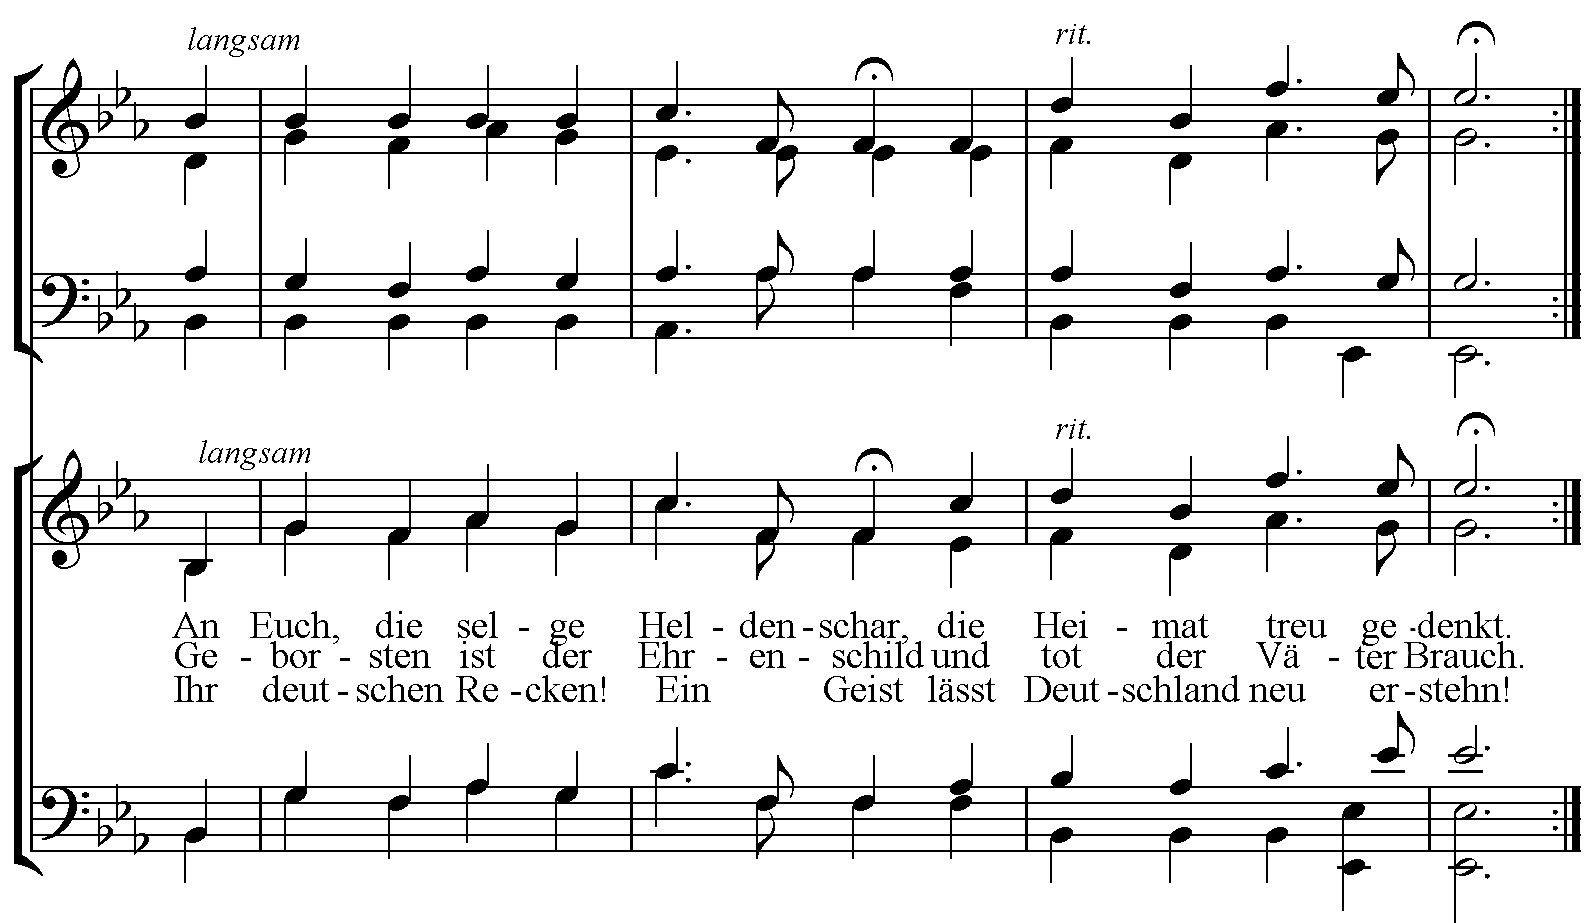
\includegraphics[width=9.827cm,height=5.713cm]{pictures/zulassungsarbeit-img103.png}

\label{bkm:Ref100248086}Abb. \stepcounter{Abb}{\theAbb}: Weihegesang
Es-Dur ,Takt 21 – 25\\
\end{supertabular}
\end{center}
Högn verzichtet in diesen Takten auf den vierstimmigen Satz und führt
alle Chorstimmen in Unisono. Der Effekt, dass alle Sänger eine Melodie
singen, suggeriert einerseits ein Gemeinschaftsgefühl, denn jeder
Zuhörer könnte sich an diesen Stellen dem Chor anschließen und wie alle
anderen Sänger „mit einer Stimme“ singen. Anderseits verleihen die
Chor-Unisoni ihren nachfolgenden Phrasen einen besonderen Ausdruck, da
durch den plötzlichen Übergang vom einstimmigen zum vierstimmigen Satz
eine große klangliche Steigerung in den nach den Unisoni folgenden
Phrasen erreicht wird. Geschickt hat Högn in der vorletzten Phrase ein
Unisono gesetzt (Abb. 101), sodass genau die letzte Phrase einer
Strophe von dieser klanglichen Bereicherung profitiert. So bleiben dem
Zuhörer vor allem die letzten und im Fall des Weihegesangs auch die für
die Botschaft wichtigsten Worte einer Strophe in Erinnerung, ganz
besonders der Schluss des Textes: \zitat{„Ein Geist
}(NS)\zitat{ lässt Deutschland neu erstehn.“}